
\documentclass[a4paper,10pt]{report}
\usepackage[utf8]{inputenc}
\usepackage[]{algorithm2e}
\usepackage[T1]{fontenc}
\usepackage{graphicx}
\usepackage{pgf,tikz}
\usepackage{caption}
\usepackage{float}
\usetikzlibrary{arrows}

\begin{document}

\section*{Decomposição k-Core}


\subsection*{Definição}
 %TODO mudar anotações para equações
Sendo G = (V,E) um grafo com n = $|V|$ vértices e m = $|E|$ arestas, dG(u) o grau do vértice u, G(C) = $(C, E|C)$ um sub-grafo de G induzido pelo subconjunto de nós C onde $E|C = \{(u,v)\subset E : u,v \subset C\} $ temos as seguintes definições relacionadas com a decomposição k-Core segundo Batagelj-Zaversnik[1]:

\begin{enumerate}
	\item Um sub-grafo G(C) é uma k-core se e só se para todos os vértices pertencentes a C o seu grau é maior ou igual a k e G(C) e G(C) é um grafo maximal.
	\item Um nó de G diz-se ter \textit{coreness} se e só se este pertence à k-core mas não a (k+1)-core.
\end{enumerate}


Assim, é possível conseguir-se as k-Cores de G removendo recursivamente todos os vértices cujo grau sejam menor que k.

Batagelj-Zaversnik[2] apresenta este algoritmo para determinar a decomposição de um grafo por k-Core:

\begin{algorithm}[H]
 \KwData{graph G = (V,L) represented by lists of neighbors Neighbors(v) for each vertex v}
 \KwResult{table core with core number core[v] for each vertex v }
 compute the degrees of vertices\;
 \ForEach{$v$ in $V$ in the order}{
  core[v] := degree[v]\;
  \ForEach{$u$ in $Neighbors(v)$ }{
		\If{ degree[u] > degree[v] }{
			degree[u] := degree[u]-1\;
			reorder V accordingly\;
		}
  }
 }
\end{algorithm}

Onde o ciclo sobre os vizinhos de $v$ simula a remoção deste vértice e o efeito disto sobre os seus vizinhos - o grau destes é reduzido por um pois deixa de existir a aresta proveniente de $v$.
Após a iteração da lista de vizinhos, os restantes vértices em $V$ devem ser reordenados de modo a garantir a ordem crescente.
%Imagem aqui


%%%Step 1%%%
\paragraph{Exemplo}
De seguida é apresentado um exemplo do algoritmo apresentado em cima. O número por debaixo dos vértices representa o seu grau($degree$) atual e a cor azul significa que a core destes vértices irão ser computadas neste passo, sequencialmente.
\begin{figure}
\definecolor{qqqqff}{rgb}{0.0,0.0,1.0}
\begin{tikzpicture}[line cap=round,line join=round,>=triangle 45,x=1.0cm,y=1.0cm]
\clip(1.5000000000000018,-2.82) rectangle (8.400000000000004,0.1);
\draw (1.9,-1.46)-- (2.96,-1.46);
\draw (5.54,-1.46)-- (6.6,-1.46);
\draw (6.6,-1.46)-- (7.98,-1.46);
\draw (2.96,-1.46)-- (4.32,-1.46);
\draw (4.32,-1.46)-- (5.54,-1.46);
\draw [shift={(4.25,-1.46)}] plot[domain=0.0:3.141592653589793,variable=\t]({1.0*1.29*cos(\t r)+-0.0*1.29*sin(\t r)},{0.0*1.29*cos(\t r)+1.0*1.29*sin(\t r)});
\draw [shift={(5.46,-1.46)}] plot[domain=3.141592653589793:6.283185307179586,variable=\t]({1.0*1.1399999999999997*cos(\t r)+-0.0*1.1399999999999997*sin(\t r)},{0.0*1.1399999999999997*cos(\t r)+1.0*1.1399999999999997*sin(\t r)});
\draw (1.920000000000002,-1.58) node[anchor=north west] {1};
\draw (3.0400000000000023,-1.56) node[anchor=north west] {3};
\draw (4.160000000000003,-1.54) node[anchor=north west] {3};
\draw (5.600000000000003,-1.54) node[anchor=north west] {3};
\draw (6.700000000000004,-1.52) node[anchor=north west] {3};
\draw (8.040000000000004,-1.54) node[anchor=north west] {1};
\begin{scriptsize}
\draw [fill=qqqqff] (1.9,-1.46) circle (1.5pt);
\draw[color=qqqqff] (2.040000000000002,-1.1800000000000002) node {$A$};
\draw [fill=black] (2.96,-1.46) circle (1.5pt);
\draw[color=black] (3.1000000000000023,-1.1800000000000002) node {$B$};
\draw [fill=black] (5.54,-1.46) circle (1.5pt);
\draw[color=black] (5.680000000000002,-1.1800000000000002) node {$D$};
\draw [fill=black] (6.6,-1.46) circle (1.5pt);
\draw[color=black] (6.740000000000003,-1.1800000000000002) node {$E$};
\draw [fill=qqqqff] (7.98,-1.46) circle (1.5pt);
\draw[color=qqqqff] (8.120000000000005,-1.1800000000000002) node {$F$};
\draw [fill=black] (4.32,-1.46) circle (1.5pt);
\draw[color=black] (4.460000000000003,-1.1800000000000002) node {$C$};
\end{scriptsize}
\end{tikzpicture}
\caption*{Começa pelos vértices A e seguidamente F, que terão a sua core[v] igual ao seu grau inicial (1), visto serem os menores.A e F afetam os vértices adjacentes B e E, respetivamente, decrementando o seus graus pois estes eram maiores. A e F deixam se ser considerados na computação.}
\end{figure}

%%%Step 2%%%
\begin{figure}
\definecolor{qqqqff}{rgb}{0.0,0.0,1.0}
\begin{tikzpicture}[line cap=round,line join=round,>=triangle 45,x=1.0cm,y=1.0cm]
\clip(1.5000000000000018,-2.82) rectangle (8.400000000000004,0.1);
\draw (1.9,-1.46)-- (2.96,-1.46);
\draw (5.54,-1.46)-- (6.6,-1.46);
\draw (6.6,-1.46)-- (7.98,-1.46);
\draw (2.96,-1.46)-- (4.32,-1.46);
\draw (4.32,-1.46)-- (5.54,-1.46);
\draw [shift={(4.25,-1.46)}] plot[domain=0.0:3.141592653589793,variable=\t]({1.0*1.29*cos(\t r)+-0.0*1.29*sin(\t r)},{0.0*1.29*cos(\t r)+1.0*1.29*sin(\t r)});
\draw [shift={(5.46,-1.46)}] plot[domain=3.141592653589793:6.283185307179586,variable=\t]({1.0*1.1399999999999997*cos(\t r)+-0.0*1.1399999999999997*sin(\t r)},{0.0*1.1399999999999997*cos(\t r)+1.0*1.1399999999999997*sin(\t r)});
\draw (1.920000000000002,-1.58) node[anchor=north west] {1};
\draw (3.0400000000000023,-1.56) node[anchor=north west] {2};
\draw (4.160000000000003,-1.54) node[anchor=north west] {3};
\draw (5.600000000000003,-1.54) node[anchor=north west] {3};
\draw (6.700000000000004,-1.52) node[anchor=north west] {2};
\draw (8.040000000000004,-1.54) node[anchor=north west] {1};
\begin{scriptsize}
\draw [fill=black] (1.9,-1.46) circle (1.5pt);
\draw[color=black] (2.040000000000002,-1.1800000000000002) node {$A$};
\draw [fill=qqqqff] (2.96,-1.46) circle (1.5pt);
\draw[color=qqqqff] (3.1000000000000023,-1.1800000000000002) node {$B$};
\draw [fill=black] (5.54,-1.46) circle (1.5pt);
\draw[color=black] (5.680000000000002,-1.1800000000000002) node {$D$};
\draw [fill=qqqqff] (6.6,-1.46) circle (1.5pt);
\draw[color=qqqqff] (6.740000000000003,-1.1800000000000002) node {$E$};
\draw [fill=black] (7.98,-1.46) circle (1.5pt);
\draw[color=black] (8.120000000000005,-1.1800000000000002) node {$F$};
\draw [fill=black] (4.32,-1.46) circle (1.5pt);
\draw[color=black] (4.460000000000003,-1.1800000000000002) node {$C$};
\end{scriptsize}
\end{tikzpicture}
\caption*{Tendo os seus graus reduzidos B e seguidamente E passam a ser os próximos elementos de $V$ a ser computados. Passando pelo mesmo processo que A e B, afetando C e D, respetivamente, reduzindo os seus graus. B e E deixam se ser considerados na computação.}
\end{figure}

\begin{figure}[H]
\definecolor{qqqqff}{rgb}{0.0,0.0,1.0}
\begin{tikzpicture}[line cap=round,line join=round,>=triangle 45,x=1.0cm,y=1.0cm]
\clip(1.5000000000000018,-2.82) rectangle (8.400000000000004,0.1);
\draw (1.9,-1.46)-- (2.96,-1.46);
\draw (5.54,-1.46)-- (6.6,-1.46);
\draw (6.6,-1.46)-- (7.98,-1.46);
\draw (2.96,-1.46)-- (4.32,-1.46);
\draw (4.32,-1.46)-- (5.54,-1.46);
\draw [shift={(4.25,-1.46)}] plot[domain=0.0:3.141592653589793,variable=\t]({1.0*1.29*cos(\t r)+-0.0*1.29*sin(\t r)},{0.0*1.29*cos(\t r)+1.0*1.29*sin(\t r)});
\draw [shift={(5.46,-1.46)}] plot[domain=3.141592653589793:6.283185307179586,variable=\t]({1.0*1.1399999999999997*cos(\t r)+-0.0*1.1399999999999997*sin(\t r)},{0.0*1.1399999999999997*cos(\t r)+1.0*1.1399999999999997*sin(\t r)});
\draw (1.920000000000002,-1.58) node[anchor=north west] {1};
\draw (3.0400000000000023,-1.56) node[anchor=north west] {2};
\draw (4.160000000000003,-1.54) node[anchor=north west] {2};
\draw (5.600000000000003,-1.54) node[anchor=north west] {2};
\draw (6.700000000000004,-1.52) node[anchor=north west] {2};
\draw (8.040000000000004,-1.54) node[anchor=north west] {1};
\begin{scriptsize}
\draw [fill=black] (1.9,-1.46) circle (1.5pt);
\draw[color=black] (2.040000000000002,-1.1800000000000002) node {$A$};
\draw [fill=black] (2.96,-1.46) circle (1.5pt);
\draw[color=black] (3.1000000000000023,-1.1800000000000002) node {$B$};
\draw [fill=qqqqff] (5.54,-1.46) circle (1.5pt);
\draw[color=qqqqff] (5.680000000000002,-1.1800000000000002) node {$D$};
\draw [fill=black] (6.6,-1.46) circle (1.5pt);
\draw[color=black] (6.740000000000003,-1.1800000000000002) node {$E$};
\draw [fill=black] (7.98,-1.46) circle (1.5pt);
\draw[color=black] (8.120000000000005,-1.1800000000000002) node {$F$};
\draw [fill=qqqqff] (4.32,-1.46) circle (1.5pt);
\draw[color=qqqqff] (4.460000000000003,-1.1800000000000002) node {$C$};
\end{scriptsize}
\end{tikzpicture}
\caption*{Finalmente é feita a computação dos cores de C e seguidamente D. Neste passo, visto que todos os seus adjacentes têm um grau igual ao seu C e D não levam a nenhuma alteração extra no grafo. Sendo que os valores atuais nos seus graus são os finais da sua core.}
\end{figure}

No final deste exemplo é criado um sub-grafo formado for B,C,D e E, sendo este uma 2-Core do grafo original.
\subsection*{Decomposição k-Core distribuída}
O algoritmo de decomposição central referido em cima requer que todo o grafo esteja em memória, o que não pode ser possível para grafos de grande escala. Devido a isto, em Distributed k-Core Decomposition, é apresentado um outro algoritmo para a decomposição k-Core distribuída.


\begin{figure}[ht!]
%\centering
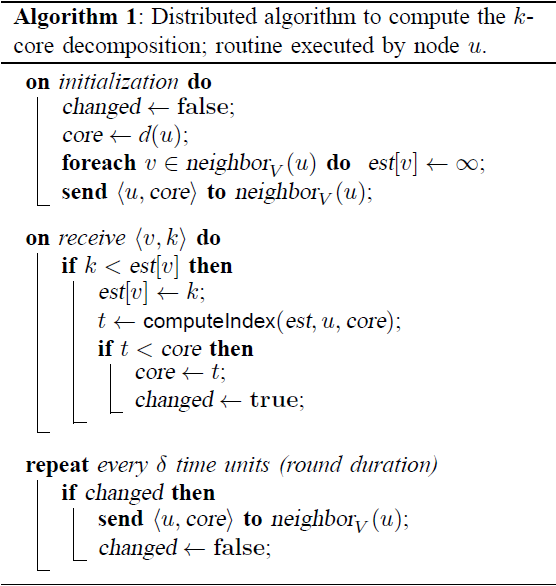
\includegraphics[width=90mm]{Algorithm1}
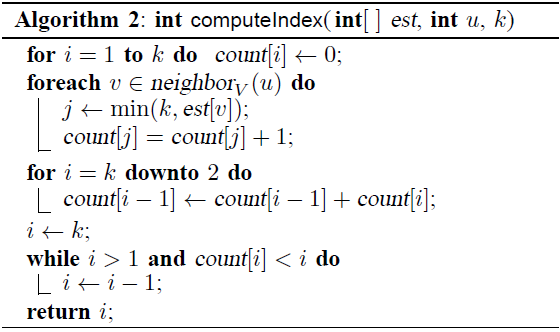
\includegraphics[width=90mm]{Algorithm2}
\label{overflow}
\end{figure}

Neste algoritmo cada vértice mantém um inteiro $core$ que mantém a estimação do seu \textit{coreness}, sendo iniciada com o seu grau. Um \textit{array} $est$ de estimativas das \textit{coreness} dos seus adjacentes, com todas as entradas iniciadas a infinito. E uma flag $changed$ que é ativa se $core$ mudar.

Cada vértice começa por enviar uma mensagem aos seus adjacentes com o seu grau inicial. 

Ao receber uma mensagem o vértice atualiza a estimativa que tem da \textit{coreness} dos seus vizinhos, caso esta seja inferior à que tem atualmente e nesse caso irá também recalcular uma nova estimativa para a sua \textit{coreness}, atualizando $core$ caso o valor desta seja menor que a do anterior. Em caso de \textit{frameworks} que implementam o modelo BSP, onde um vértice pode receber várias mensagens de uma vez basta calcular a estimativa do vértice uma única vez depois de atualizar a estimativa dos vizinhos.

Após o recalculo, de tempo em tempo para evitar excesso de mensagens, se a $core$ ter sido alterada esta é enviada aos seus vizinhos. Tal como se passava na computação da estimativa no caso de \textit{frameworks} que implementam o modelo BSP, visto que estas apresentam sincronização por barreira, a nova $core$ pode ser enviado sempre que ocorrer uma alteração. Este algoritmo para quando todos os valores convergirem ( a $core$ de nenhum vértice é alterada).
%Distributed k-Core Decomposition

%http://arxiv.org/pdf/1103.5320v2.pdf

%http://arxiv.org/pdf/cs/0310049v1.pdf
\end{document}